\documentclass[12pt,oneside]{udthesis}
\usepackage[]{graphicx}\usepackage[]{color}
% maxwidth is the original width if it is less than linewidth
% otherwise use linewidth (to make sure the graphics do not exceed the margin)
\makeatletter
\def\maxwidth{ %
  \ifdim\Gin@nat@width>\linewidth
    \linewidth
  \else
    \Gin@nat@width
  \fi
}
\makeatother

\definecolor{fgcolor}{rgb}{0.345, 0.345, 0.345}
\newcommand{\hlnum}[1]{\textcolor[rgb]{0.686,0.059,0.569}{#1}}%
\newcommand{\hlstr}[1]{\textcolor[rgb]{0.192,0.494,0.8}{#1}}%
\newcommand{\hlcom}[1]{\textcolor[rgb]{0.678,0.584,0.686}{\textit{#1}}}%
\newcommand{\hlopt}[1]{\textcolor[rgb]{0,0,0}{#1}}%
\newcommand{\hlstd}[1]{\textcolor[rgb]{0.345,0.345,0.345}{#1}}%
\newcommand{\hlkwa}[1]{\textcolor[rgb]{0.161,0.373,0.58}{\textbf{#1}}}%
\newcommand{\hlkwb}[1]{\textcolor[rgb]{0.69,0.353,0.396}{#1}}%
\newcommand{\hlkwc}[1]{\textcolor[rgb]{0.333,0.667,0.333}{#1}}%
\newcommand{\hlkwd}[1]{\textcolor[rgb]{0.737,0.353,0.396}{\textbf{#1}}}%
\let\hlipl\hlkwb

\usepackage{framed}
\makeatletter
\newenvironment{kframe}{%
 \def\at@end@of@kframe{}%
 \ifinner\ifhmode%
  \def\at@end@of@kframe{\end{minipage}}%
  \begin{minipage}{\columnwidth}%
 \fi\fi%
 \def\FrameCommand##1{\hskip\@totalleftmargin \hskip-\fboxsep
 \colorbox{shadecolor}{##1}\hskip-\fboxsep
     % There is no \\@totalrightmargin, so:
     \hskip-\linewidth \hskip-\@totalleftmargin \hskip\columnwidth}%
 \MakeFramed {\advance\hsize-\width
   \@totalleftmargin\z@ \linewidth\hsize
   \@setminipage}}%
 {\par\unskip\endMakeFramed%
 \at@end@of@kframe}
\makeatother

\definecolor{shadecolor}{rgb}{.97, .97, .97}
\definecolor{messagecolor}{rgb}{0, 0, 0}
\definecolor{warningcolor}{rgb}{1, 0, 1}
\definecolor{errorcolor}{rgb}{1, 0, 0}
\newenvironment{knitrout}{}{} % an empty environment to be redefined in TeX

\usepackage{alltt}
\newcommand{\SweaveOpts}[1]{}  % do not interfere with LaTeX
\newcommand{\SweaveInput}[1]{} % because they are not real TeX commands
\newcommand{\Sexpr}[1]{}       % will only be parsed by R



%----------------------------------------------------------------------------------------
%	Atributes Settings
%----------------------------------------------------------------------------------------
% About your study degree programme
\def \study{ITM} % possible options: ITM, SWD, MSD, IRM, IMS

% More about you and your thesis:
\def \Title{TESIS}
\def \title{PRA TESIS}
\def \subtitle{Preferensi Pengunjung Waterfront di Kota Parepare Sebagai Kota Wisata}
\def \yourName{Muhammad Uliah Shafar}
\def \yourIdentifier{21020119420029}
\def \yourPlace{<place>}
\def \submissionDate{<date>}  % month year. e.g. June 2017
\DTMsavedate{tanggalberita}{2021-01-31} %tanggal sidang
\def \hariBerita{<day>} %hari sidang
\def \yourAdvisor{Dr. Ars. Ir. Wijayanti, M.Eng}
\DTMsavetime{waktuberita}{24:60:60} %waktu sidang
\def \yourNipAdvisor{196307111990012001}
\def \yourSecAdvisor{Prof. Dr. Ir. Atik Suprapti,  M.T.}
\def \yourNipSecAdvisor{196511131998032001}
%\def \thisDocumentIsA{Thesis} % possible options:
                     % Thesis  .... for Master's Thesis   / Masterarbeit
                     % Thesis  .... for Bachelor's Thesis / Bachelorarbeit
                     % Seminar .... for Seminar Work      / Seminararbeit
                     % Project .... for Project Work      / Projektarbeit

% ITM/SWD/IRM: you could possibly write in German.
%\def \yourLanguage{english} % possible options: german, english






\begin{document}
% Child with Latex code only:


%--------------------------------------------------------------------------------------
% R chunk
%--------------------------------------------------------------------------------------
% Set parent


% load stat

%------------------------------------------------------

%------------------------------------------------------



\newcommand{\pieChartFig}
{\begin{figure}[h]
\centering

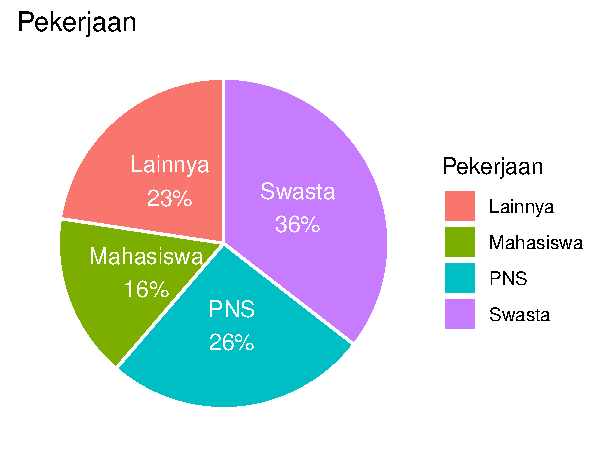
\includegraphics[width=\maxwidth]{../figures/stats2-1} 
\caption{Pie Chart Pekerjaan}
\label{pieChartFig}\end{figure}
}



\newcommand{\tabRegresi}{
% latex table generated in R 4.0.3 by xtable 1.8-4 package
% Fri Mar 19 20:37:13 2021
\begin{table}[ht]
\centering
\begin{tabular}{lrrrrr}
  \hline
 & Df & Sum Sq & Mean Sq & F value & Pr($>$F) \\ 
  \hline
data2\$total\_fit & 1.000 & 96.998 & 96.998 & 3.679 & 0.065 \\ 
  Residuals & 29.000 & 764.551 & 26.364 &  &  \\ 
   \hline
\end{tabular}
\caption{Regresi Linear} 
\label{tabRegresi}
\end{table}
}

%--------------------------------------------------------------------------------------


\chapter{Pendahuluan}\label{chap:pendahuluan}

\section{Latar Belakang}
\cite{imansari2015}
\lipsum[2-4]

\section{Rumusan Masalah}
\lipsum[2-4]

\begin{enumerate}
    \item  Lorem Ipsum ?
    \item Lorem Ipsum ?
\end{enumerate}


\section{Tujuan Penelitian}
\lipsum[2-4]
\section{Manfaat Penelitian}

\lipsum[2-4]
\begin{enumerate}
\item Lorem Ipsum
\item Lorem Ipsum
\end{enumerate}


\section{Sistematika Penulisan}
\lipsum[1-1]
\begin{itemize}
	\item Bab 1 : Pendahuluan\\
Bab terdiri dari latar belakang permasalahan, perumusan masalah, tujuan penelitian, manfaat penelitian, dan sistematika penulisan.
	\item Bab 2 : Tinjauan Pustaka\\
Bab ini terdiri dari landasan teori yang digunakan untuk memperkuat penemuan masalah, penelitian terdahulu dan kerangka pemikiran.
	\item Bab 3 : Metodologi Penelitian\\
Bab ini terdiri dari penjelasan variabel dan jenis paradigma yang digunakan untuk mencapai penemuan sesuai rumusan masalah, populasi, sampel, dan cara pengumpulan data.
	\item Bab 4 : Hasil dan Pembahasan\\
Bab ini terdiri dari pembahasan mengenai hasil - hasil penelitian yang berupa data-data yang didapatkan, dengan melakukan pengolahan terhadap indikator-indikator kenyamanan. Setelah pengelolahan bahan-bahan tersebut, analisis diperlukan untuk menemukan penemuan penelitian. Analisis diarahkan untuk menjawab rumusan masalah.
	\item Bab V : Kesimpulan\\
Bab terakhir terdiri dari kesimpulan yang didapatkan dari analisis terhadap permasalahan yang terdapat pada penelitian ini, sehingga penemuan bersama saran-saran dari penelusi dapat menghasilkan apa yang diinginkan.


\end{itemize}
\begin{comment}
\section{Alur Pikir}

\begin{figure}[ht]
\centering
\begin{tikzpicture}[node distance=2cm]
\node (ltr) [startstop] {Latar Belakang};

\node (rum) [startstop, right of=ltr, xshift=2cm] {Perumusan Masalah};

\node (tuj) [startstop, below of=rum, yshift=0.5cm] {Tujuan Penelitian};


\node (pus) [startstop, below of=tuj, yshift=0.5cm] {Studi Pustaka};


\node (kaj) [startstop, below of=pus, text width=3.5cm, xshift= -4cm, yshift=.5cm] {
	\textbf{Kajian Teori}\\ - Fitur binaan\\ - Aktivitas Luar
};


\node (kaj2) [startstop, below of=pus, text width=3.5cm, xshift= 4cm, yshift=.5cm] {
	\textbf{Gambaran Objek}\\ Fitur Binaan dan Aktivitas Luar Jl. Pinggir Laut
};


\node (hip) [startstop, below of=pus, yshift=-.5cm] {Hipotesa};


\node (met) [startstop, below of=hip, yshift=-.75cm, text width=7cm] {
	\textbf{Metode Peneltian}\\ Menggunakan Metode penelitian Kuantitatif Rasionalistik

	\textbf{Variabel}\\
	- Bebas : Fitur Binaan\\
	- Terikat : Aktivitas Luar\\

	\textbf{Sumber data}: Observasi dan Kuesioner
};

\node (ana) [startstop, below of=met, text width=8cm, yshift=-2cm] {
		\textbf{Analisis Data Statistik}\\ Penelitian ini menggunakan metode statika berupa uji regresi guna mengetahui pengaruh variabel fitur binaan terhadap variabel aktivitas luar.
};

\node (tem) [startstop, below of=ana, yshift=-.25cm] {Temuan Penelitian};

\node (kes) [startstop, below of=tem, yshift=.6cm] {Kesimpulan dan Rekomendasi};

\draw [arrow] (ltr) -- (rum);
\draw [arrow] (rum) -- (tuj);
\draw [arrow] (tuj) -- (pus);

\draw [arrow] (pus) -| (kaj);
\draw [arrow] (pus) -| (kaj2);

\draw [doublearrow] (kaj) -- (kaj2);

\draw [arrow] (kaj) |- (met);
\draw [dotted] (kaj) |- (hip);

\draw [arrow] (kaj2) |- (met);
\draw [dotted] (kaj2) |- (hip);

\draw [arrow] (met) -- (ana);
\draw [arrow] (ana) -- (tem);

\draw [arrow] (tem) -- (kes);

\end{tikzpicture}
\caption{Alur Pikir}
\end{figure}
\end{comment}
\newpage

\chapter{Tinjauan Pustaka}\label{chap:pstk}

\lipsum[2-4]

\section{Kerangka Penelitian}


Dari hasil tinjauan pustaka peneliti menyusun kerangka penelitian berdasarkan variabel-variable yang layak diteliti.


\begin{figure}[htbp]
\centering
\begin{tikzpicture}[node distance=2cm]

	\node (tit) [startstop, text width= 5cm] {Fitur Fisik Binaan pada Aktivitas Luar Jl. Pinggir Laut};

	\node (va1) [startstop, below of=tit, text width=5cm, xshift=-3cm] {Variabel Bebas\\ Fitur Fisik Binaan};

	\node (va2) [startstop, below of=tit, text width=5cm, xshift=3cm] {Variabel Tergantung\\ Aktivitas Luar};

	\node (de1) [startstop, below of=va1, text width=5cm, yshift=-2cm] {
		\textbf{Sub Variabel Bebas}\\
		- Elemen Jalan \\
		- Kualitas Jalan \\
		- Elemen Tempat Duduk \\
		- Kualitas Tempat Duduk \\
		- Elemen Alami \\
		- Kualitas Alami \\
		- Fasilitas \& Aminities \\
		- Estetika \\

	};
	\node (de2) [startstop, below of=va2, text width=5cm, yshift=-2cm] {
			\textbf{Sub Variable Tergantung}\\
		- Aktivitas relaxsasi\\
		- Aktivitas fisik\\
		- Travel aktif\\
		- Interaction with wildlife and nature\\
		- Interaksi sosial\\
		- Partisipasi di aktivitas grup\\
		};
\draw [arrow] (tit) -| (va1);
\draw [arrow] (va1) -- (de1);
\draw [arrow] (tit) -| (va2);
\draw [arrow] (va2) -- (de2);

\end{tikzpicture}
\caption{Alur Pikir}
\end{figure}

\chapter{Metodologi Penelitian}\label{chap:method}

\section{Metode dan Jenis Penelitian}

\lipsum[2-4]

\section{ Knitr child Documents}
You should note that using knitr package you can easily incorporate difference kinds of files into a project.

\tabRegresi
\pieChartFig

\chapter{Kesimpulan}\label{chap:kesimp}
\bibliographystyle{apalike}
\bibliography{bibliography/biblio.bib}
\end{document}
